\section{Triển khai và vận hành}
\subsection{Triển khai Frontend}
\textbf{Bước 1: Đăng nhập Vercel}

Truy vập vercel.com và sử dụng tài khoản GitHub để đăng nhập

\textbf{Bước 2: Tạo dự án mới}

Chọn \textbf{Add New} -> \textbf{Project}
\begin{figure}[H]
    \centering
    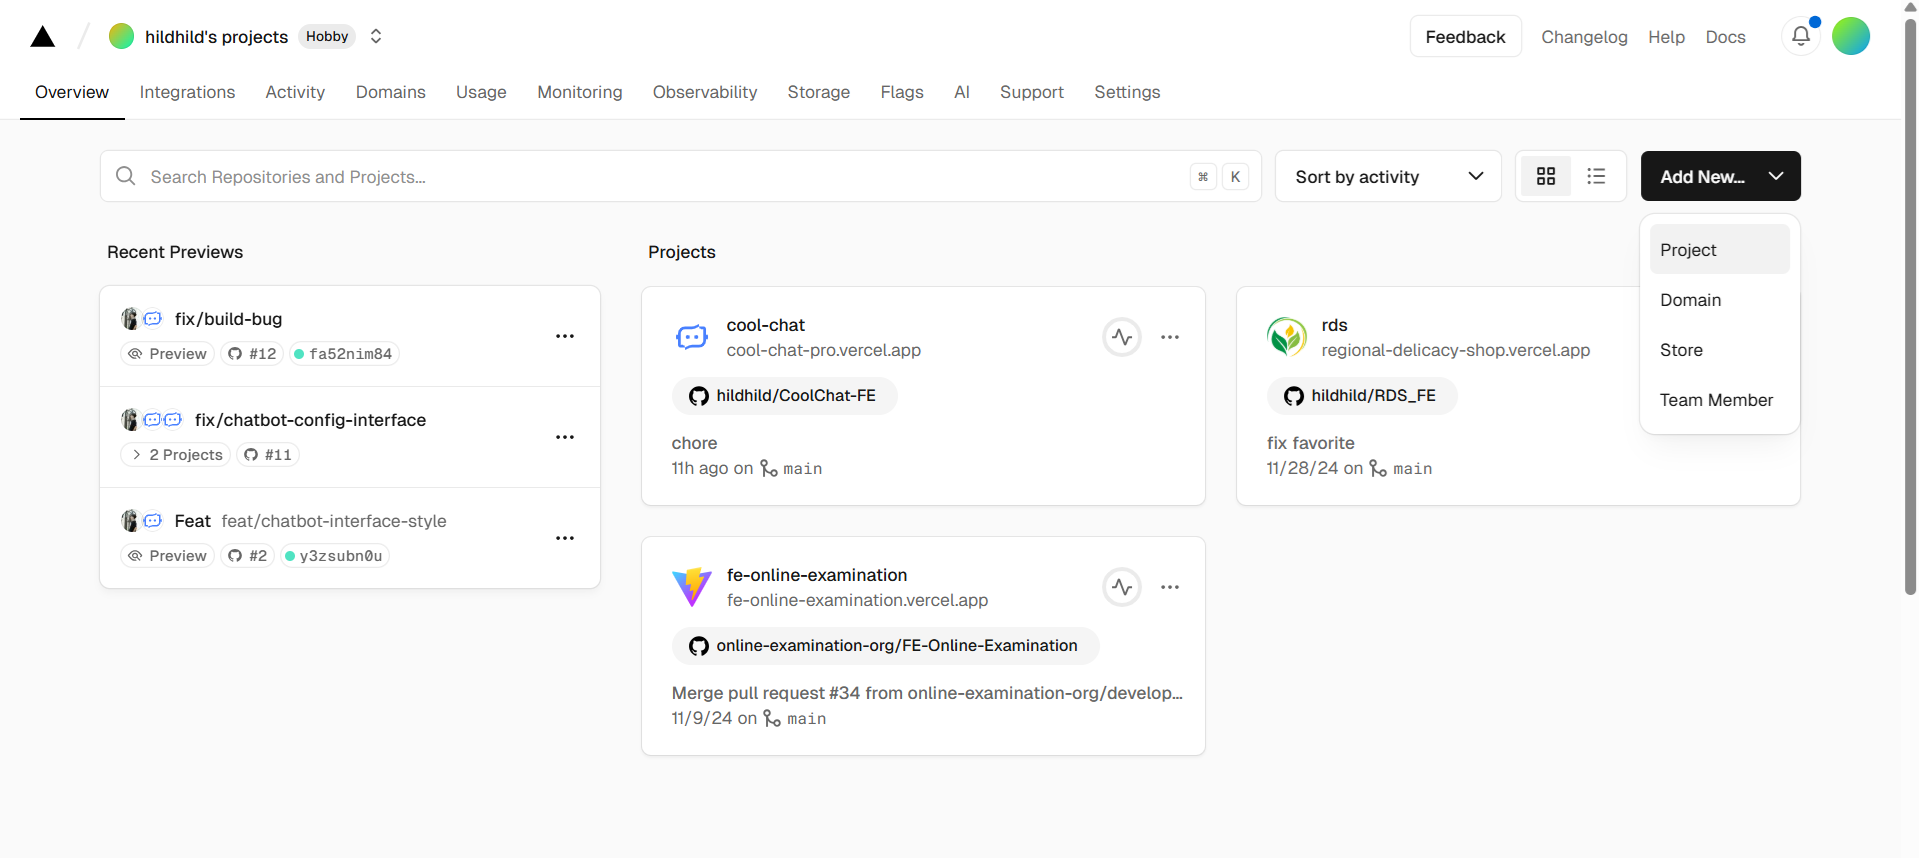
\includegraphics[width=\textwidth]{Images/Deployment/vercel1.png}
    \vspace{0.5cm}
    \caption{Tạo dự án mới trên Vercel}
    \label{fig:enter-label}
\end{figure}

\textbf{Bước 3: Nhập repository}  

Nhập Git repository cần triển khai, ở đây nhóm sẽ chọn CoolChat-FE
\begin{figure}[H]
    \centering
    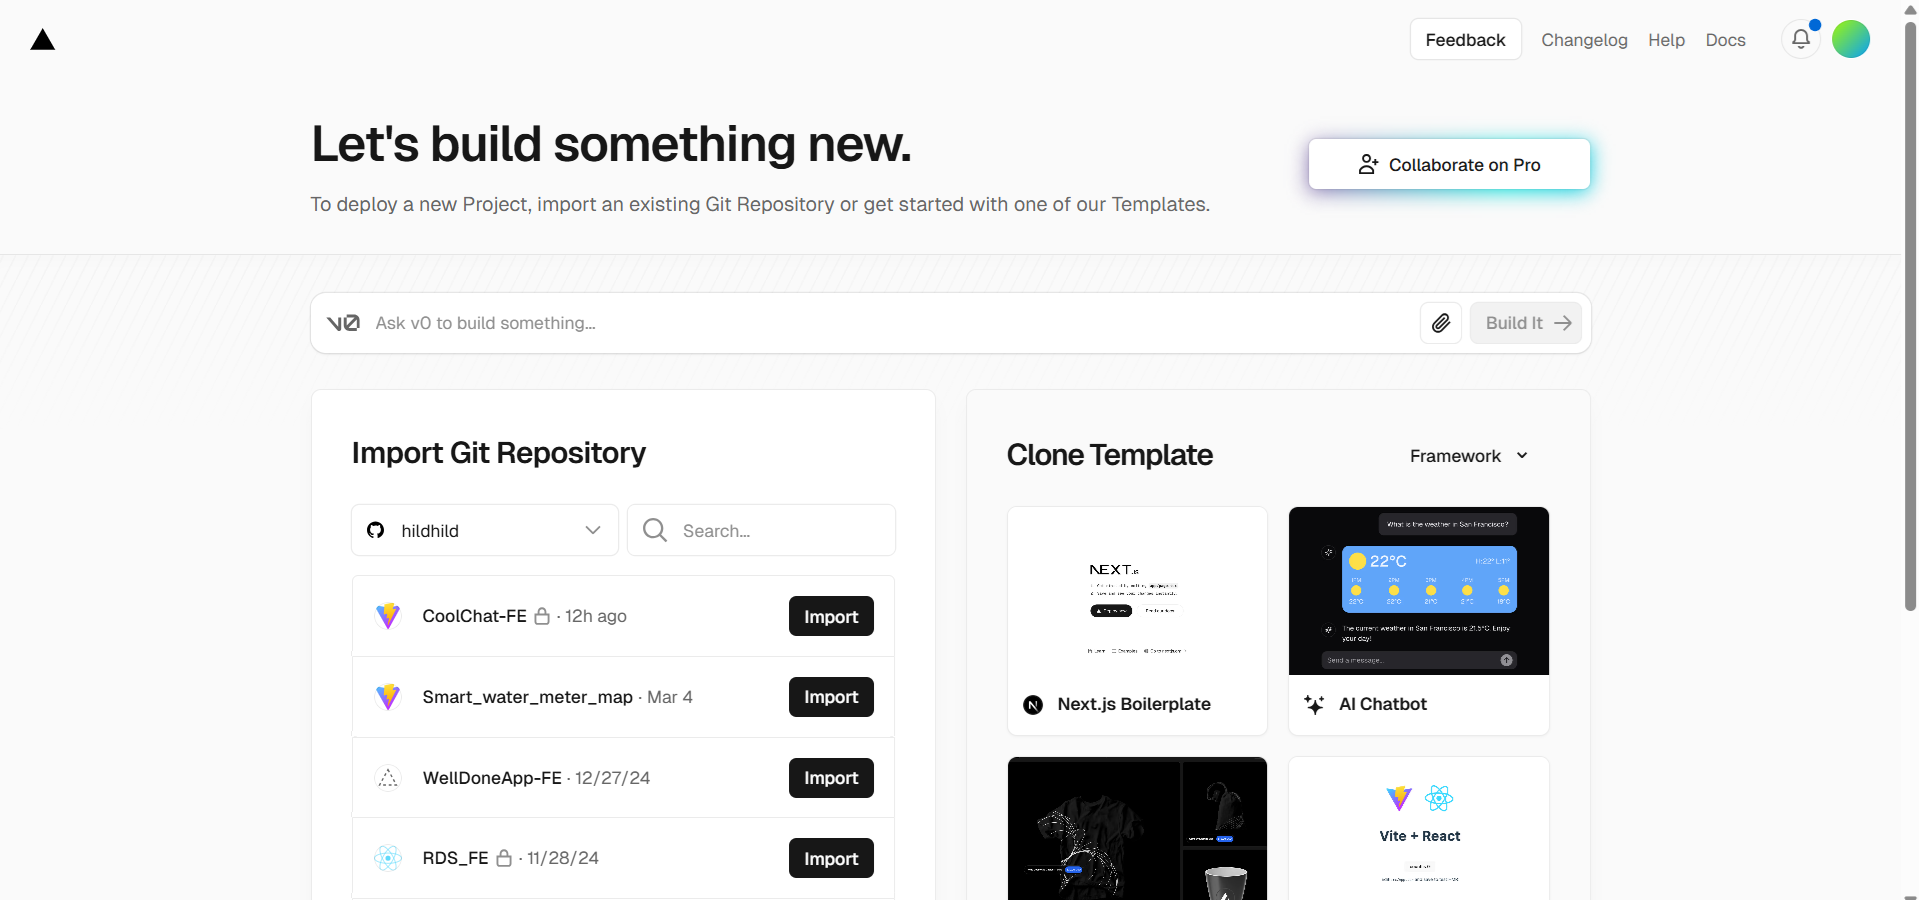
\includegraphics[width=\textwidth]{Images/Deployment/vercel2.png}
    \vspace{0.5cm}
    \caption{Nhập repository trên Vercel}
    \label{fig:enter-label}
\end{figure}

\textbf{Bước 4: Cấu hình cài đặt}  

Bao gồm
\begin{itemize}
    \item Thiết lập build và output
    \item Cài đặt các biến môi trường (environment variables)
\end{itemize}
\begin{figure}[H]
    \centering
    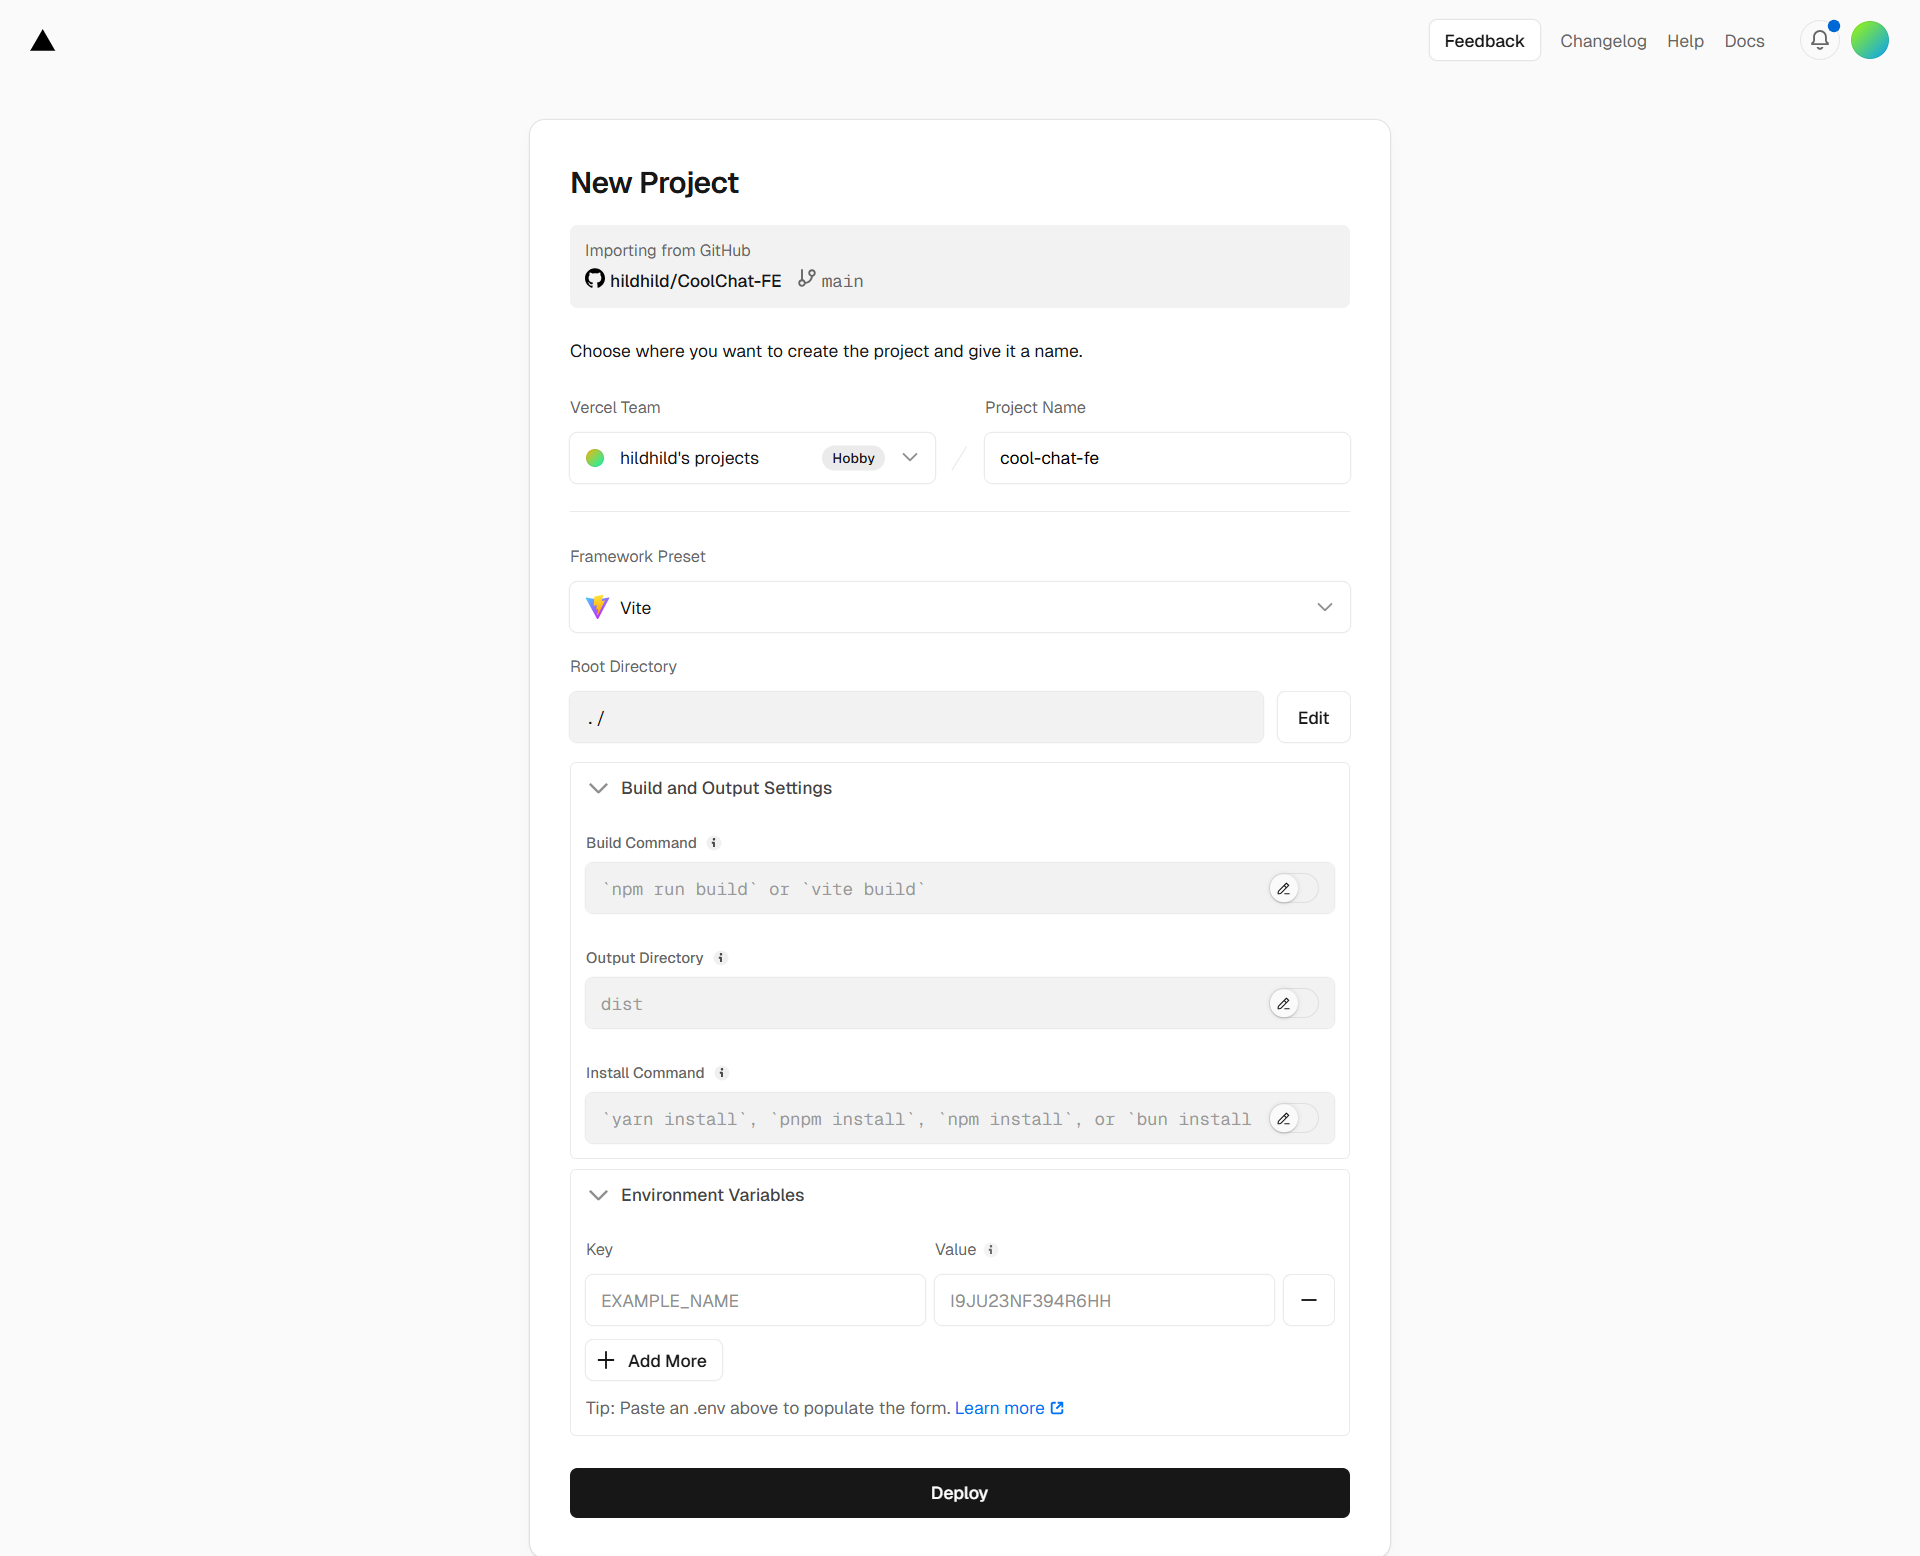
\includegraphics[width=\textwidth]{Images/Deployment/vercel3.png}
    \vspace{0.5cm}
    \caption{Cấu hình cài đặt dự án trên Vercel}
    \label{fig:enter-label}
\end{figure}

\textbf{Bước 5: Triển khai dự án}

Chọn \textbf{Deploy} để triển khai dự án. Vercel sẽ tạo Dự án và triển khai dựa trên các cấu hình đã chọn.  

\textbf{Bước 6: Triển khai thành công}

Màn hình hiển thị Domain cho dự án. Trang này sẽ có thể thấy bởi bất cứ ai có URL.
\begin{figure}[H]
    \centering
    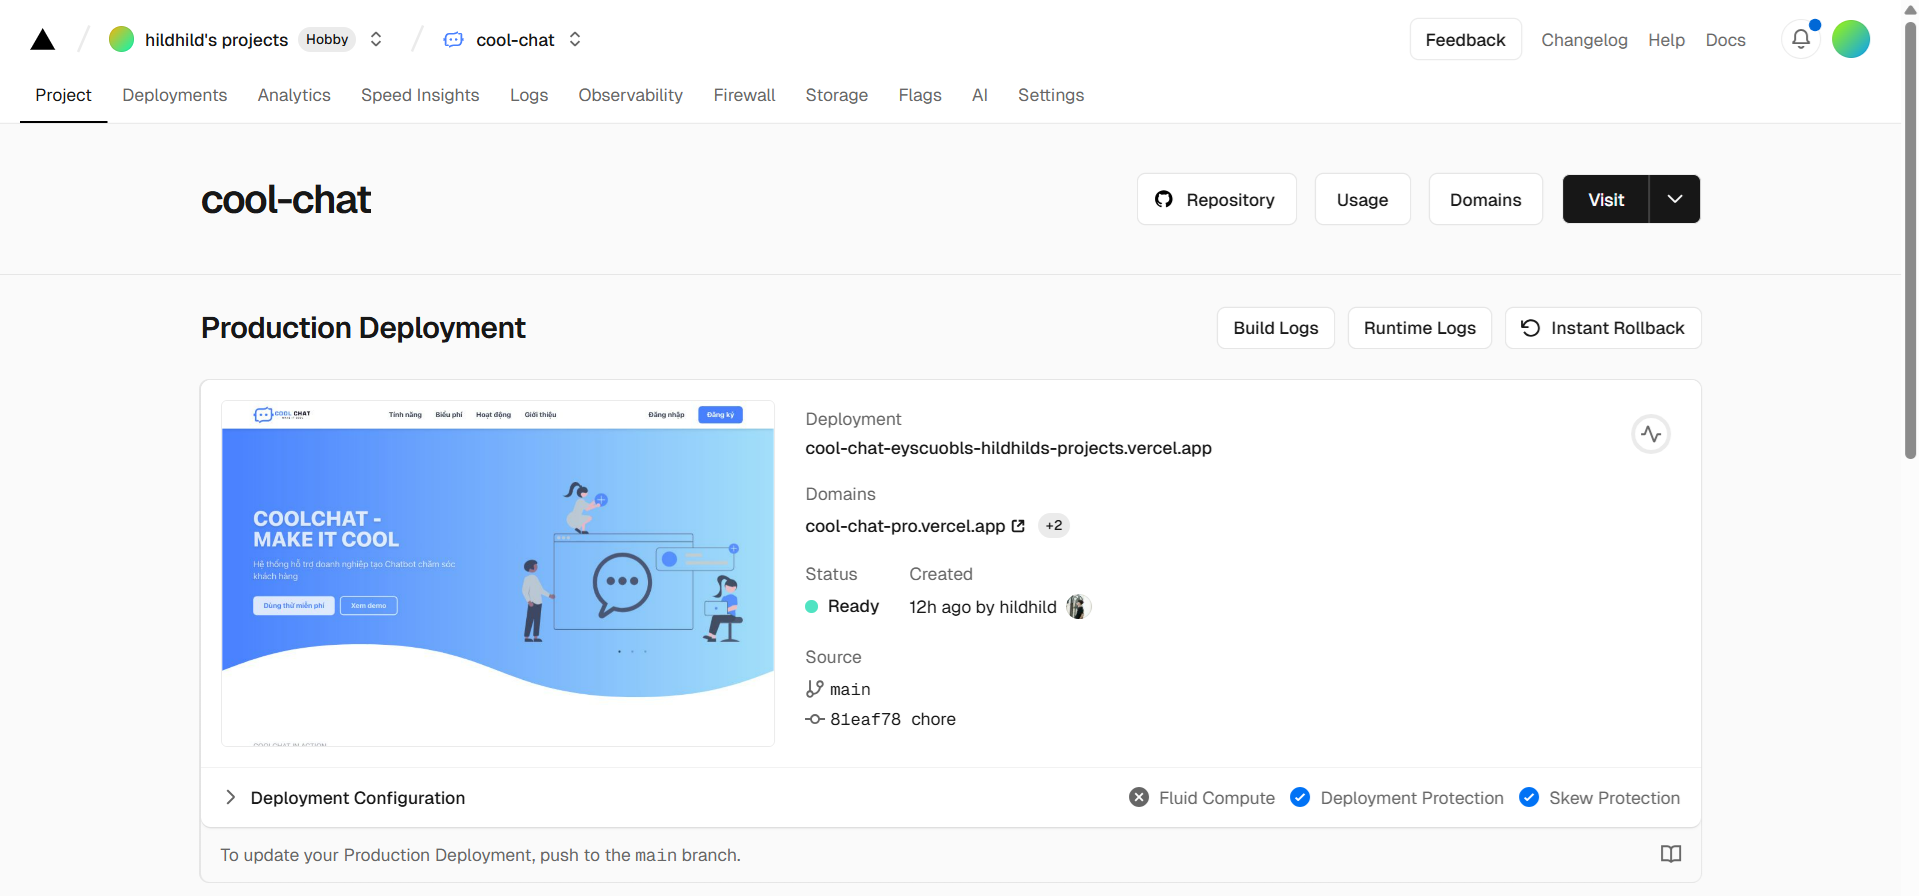
\includegraphics[width=\textwidth]{Images/Deployment/vercel4.png}
    \vspace{0.5cm}
    \caption{Kết quả triển khai trên Vercel}
    \label{fig:enter-label}
\end{figure}
\begin{figure}[H]
    \centering
    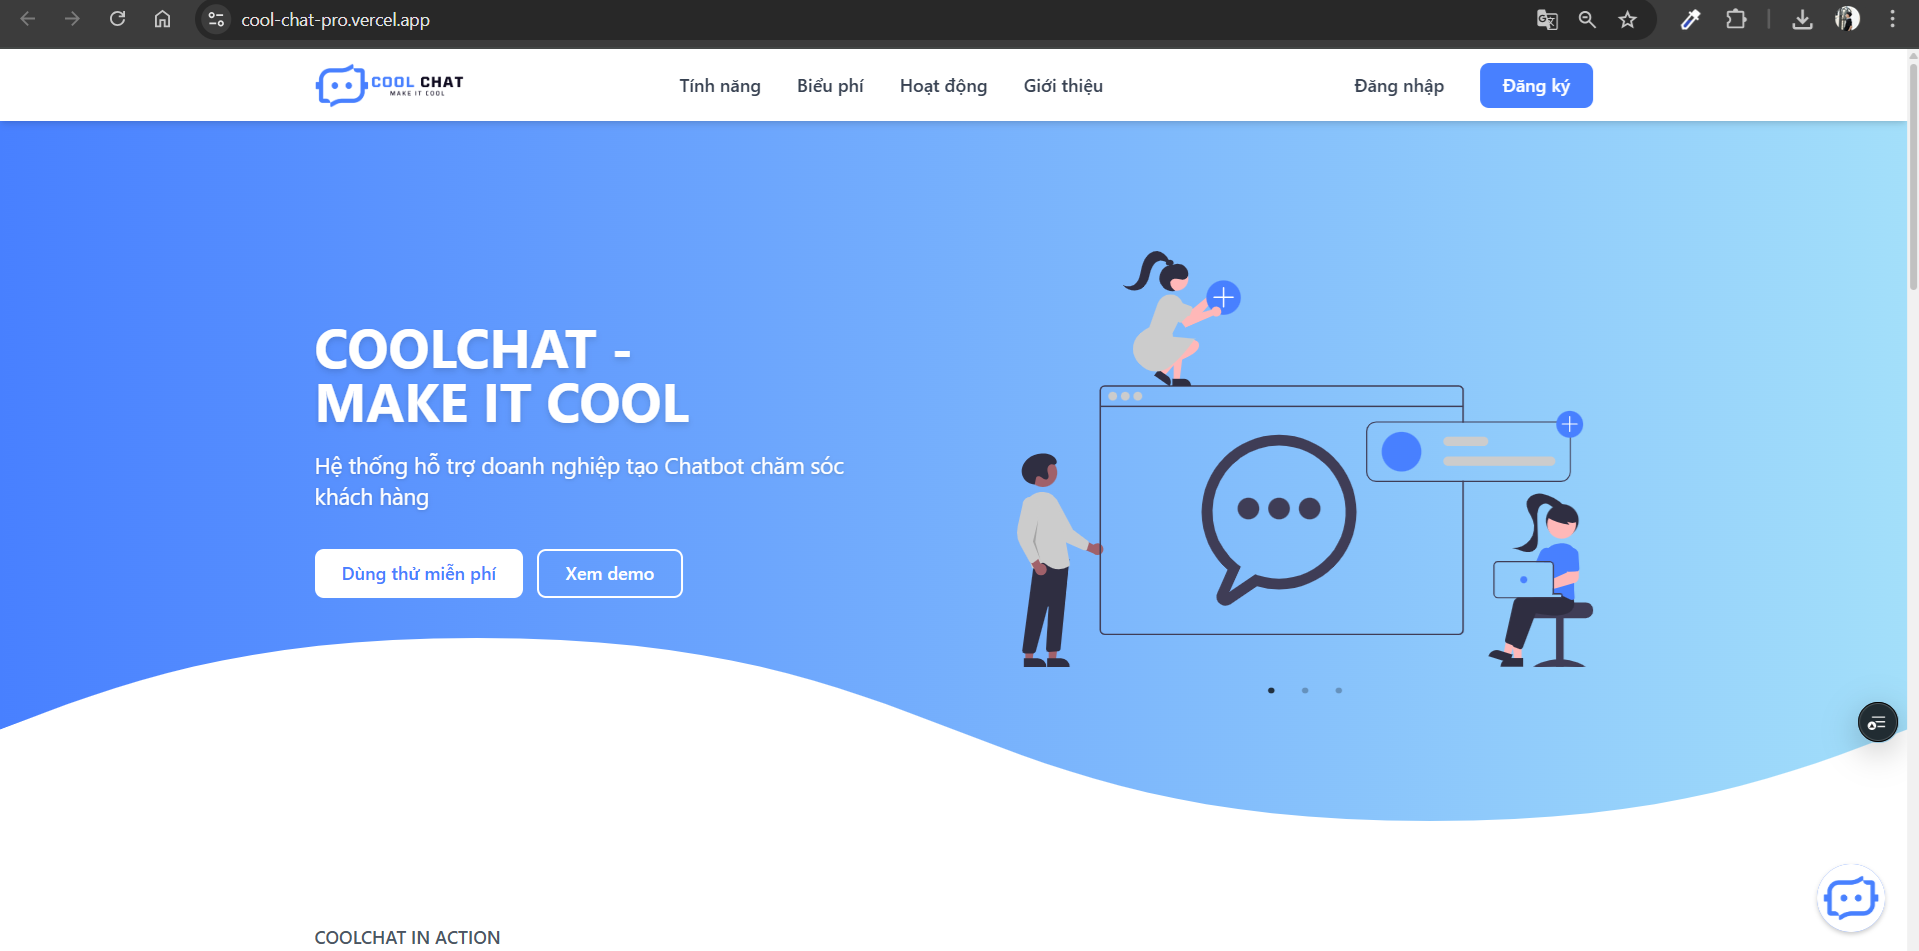
\includegraphics[width=\textwidth]{Images/Deployment/vercel5.png}
    \vspace{0.5cm}
    \caption{Vào URL của dự án đã triển khai bằng Vercel}
    \label{fig:enter-label}
\end{figure}

\textbf{Bước 7: Cập nhật và quản lý}
\begin{itemize}
    \item Tự động cập nhật: Khi push code lên GitHub nhánh main, Vercel sẽ tự build và cập nhật phiên bản mới.
    \item Kiểm tra trạng thái: Quản lý dự án tại trang Dashboard của Vercel.
\end{itemize}
\begin{figure}[H]
    \centering
    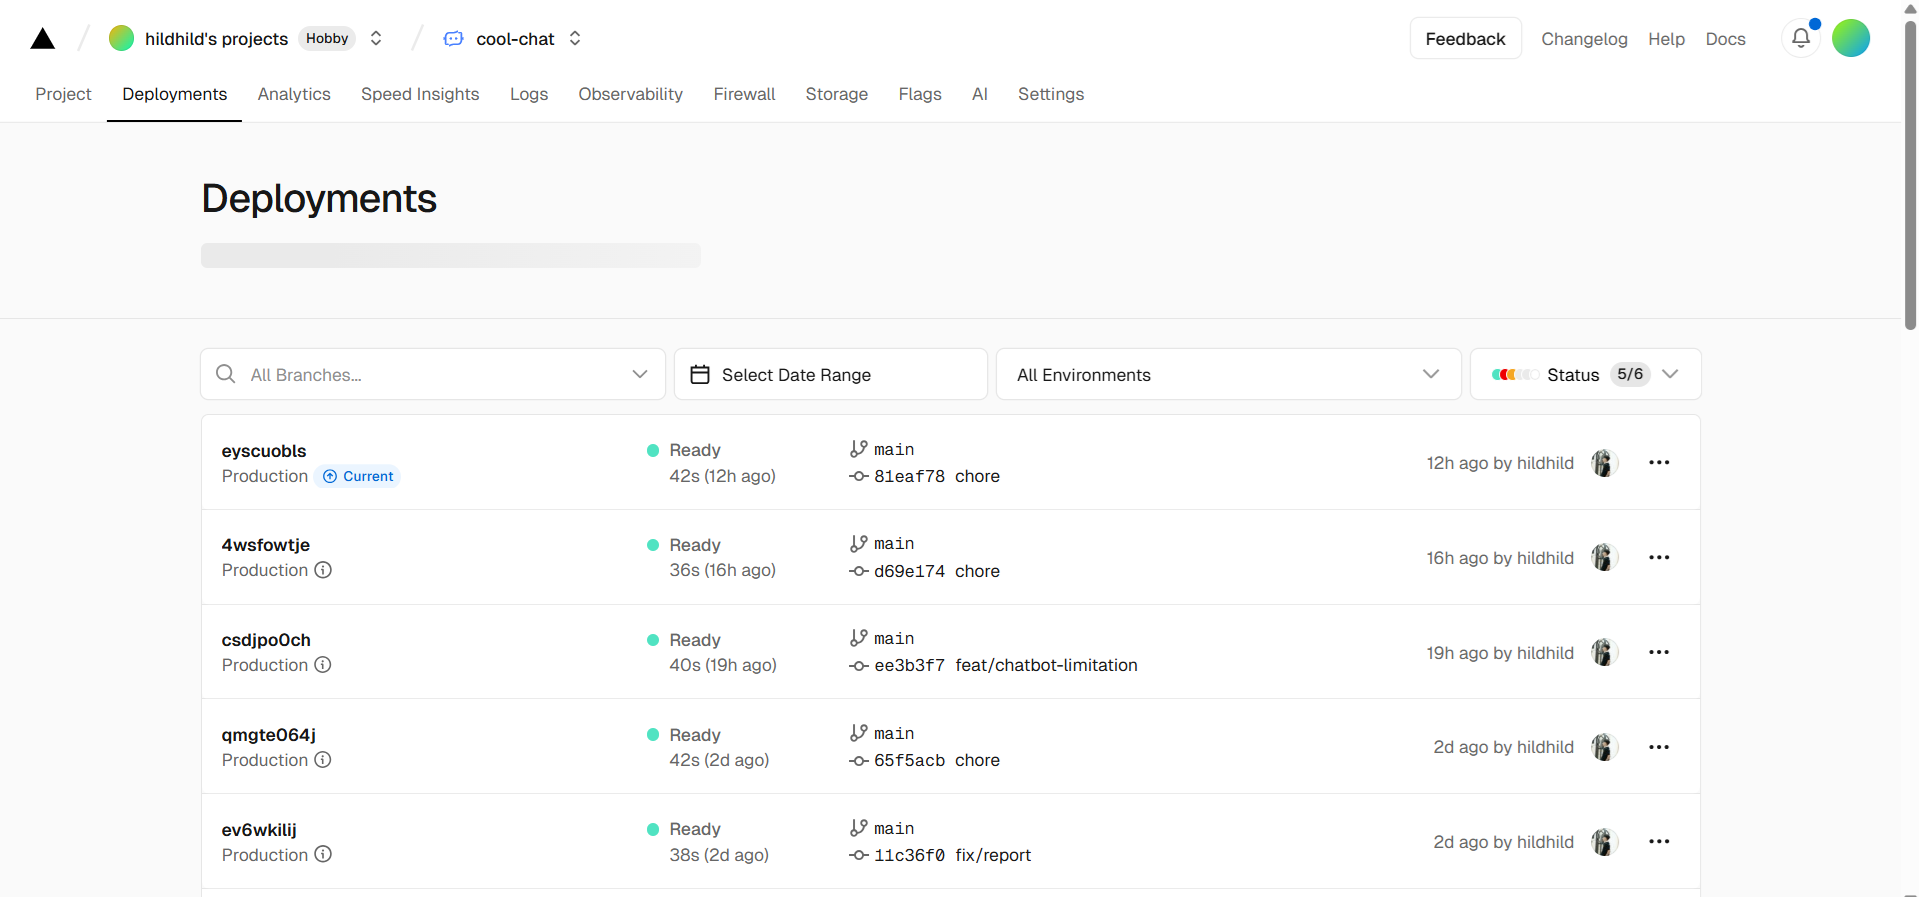
\includegraphics[width=\textwidth]{Images/Deployment/vercel6.png}
    \vspace{0.5cm}
    \caption{Quản lý các phiên bản trên Vercel}
    \label{fig:enter-label}
\end{figure}